Auf die Diagramme folgt jeweils eine textuelle Beschreibung aller Endpunkte. \\
Darin stellen Pfadteile in angle brackets (\texttt{<x>}) nötige, und Pfadteile in square brackets (\texttt{[x]}) optionale Parameter dar.\\

\section{API-Diagramme für Lehrer}
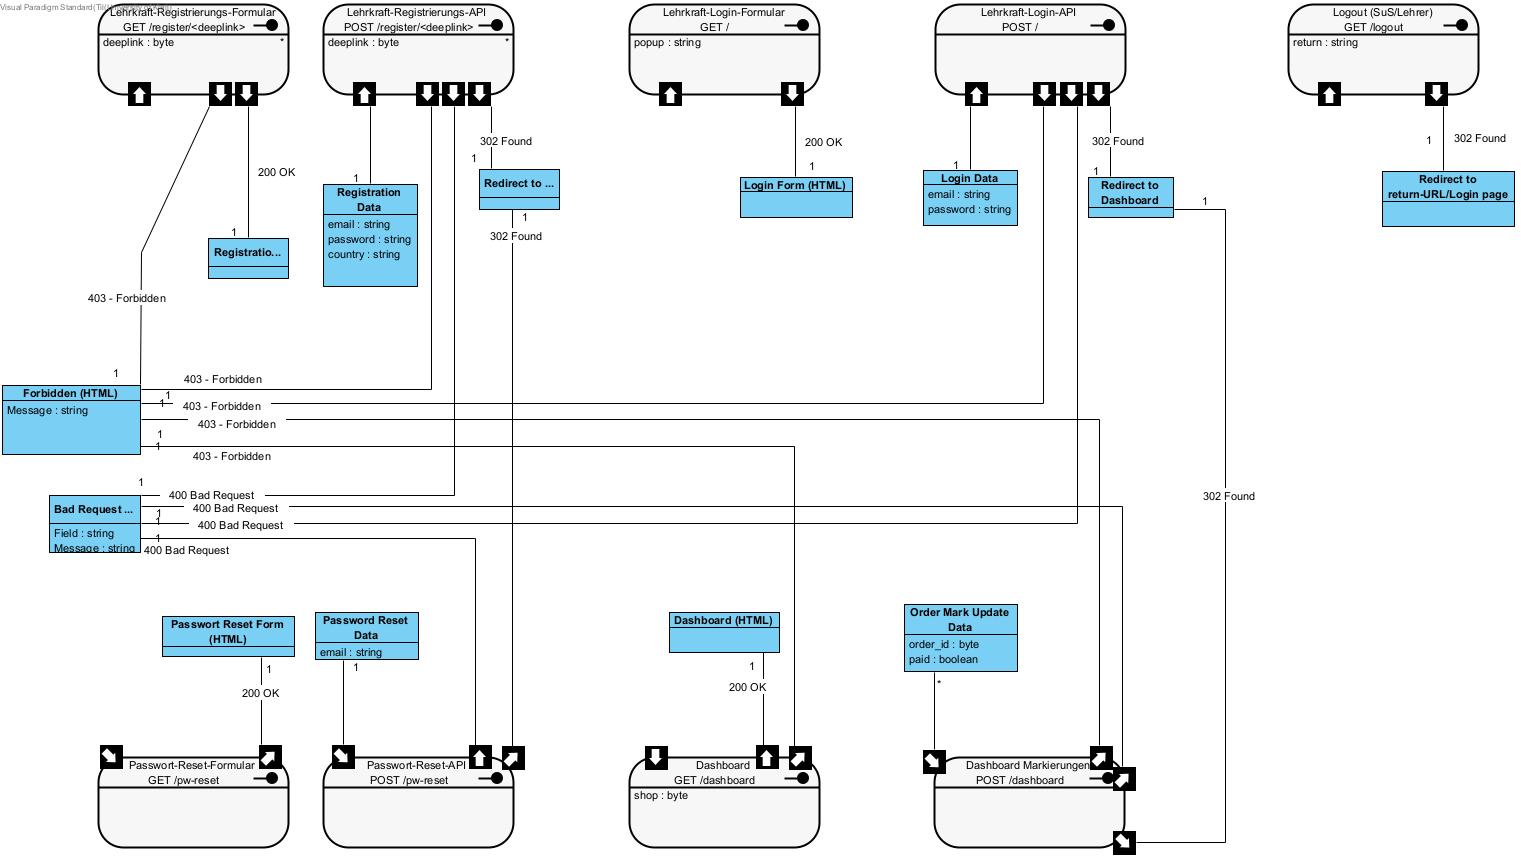
\includegraphics[width=\textwidth]{img/api-lehrkraft-login}
\begin{itemize}
	\item \texttt{/register/<deeplink>}: Die Lehrer-Registrierung ist nur über deinen Deeplink erreichbar.
		\begin{itemize}
			\item GET: Registrierungsformular.
			\item POST: Hier wird ein JSON-Body mit den Daten aus dem Registrierungsformular erwartet. Erfolg führt zu einer Weiterleitung zu \texttt{/?popup=Registrierung+Erfolgreich}.
		\end{itemize}
	\item \texttt{/?[popup=<TEXT>]}: Lehrkraft-Login.
		\begin{itemize}
			\item GET: Login-Formular. Falls ein popup-Text gegeben wird, wird dieser angezeigt.
			\item POST: Hier wird ein JSON-Body mit Login-Daten erwartet. Erfolg führt zu einer Weiterleitung zu \texttt{/dashboard}.
		\end{itemize}
	\item \texttt{/pw-reset}: Lehrkraft-Passwort-Reset.
		\begin{itemize}
			\item GET: Passwort-Reset-Formular.
			\item POST: Hier wird ein JSON-Body mit der E-Mail, dessen zugehöriger Account sein Passwort zurückgesetzt haben soll, erwartet. Erfolg führt zu einer Weiterleitung zu \texttt{/}.
		\end{itemize}
	\item \texttt{/logout?[return=<URL>]}: Logout.
		\begin{itemize}
			\item GET: Aufruf führt zum Logout, sowohl von Lehrkraft- als auch SuS-Sessions. Falls angegeben, wird danach zur return-URL weitergeleitet, sonst zu \texttt{/}.
		\end{itemize}
	\item \texttt{/dashboard?[shop=<ID>]}: Lehrkraft-Dashboard. Nur nach Login mit Lehreraccount erreichbar. Angabe des shop-parameters filtert die angezeigte Bestellungsliste auf Bestellungen bei dem gegebenen Shop.
		\begin{itemize}
			\item GET: Lehrkraft-Dashboard. Es werden nur Daten zu den Großhändlern aus dem Land des Lehrkraftaccounts dargestellt.
			\item POST: Hier wird ein JSON-Body erwartet, der für eine Untermenge an Bestellungen angibt, ob sie als bezahlt oder unbezahlt zu markieren sind. Erfolg führt zu einer Weiterleitung zu \texttt{/dashboard}.
		\end{itemize}
\end{itemize}

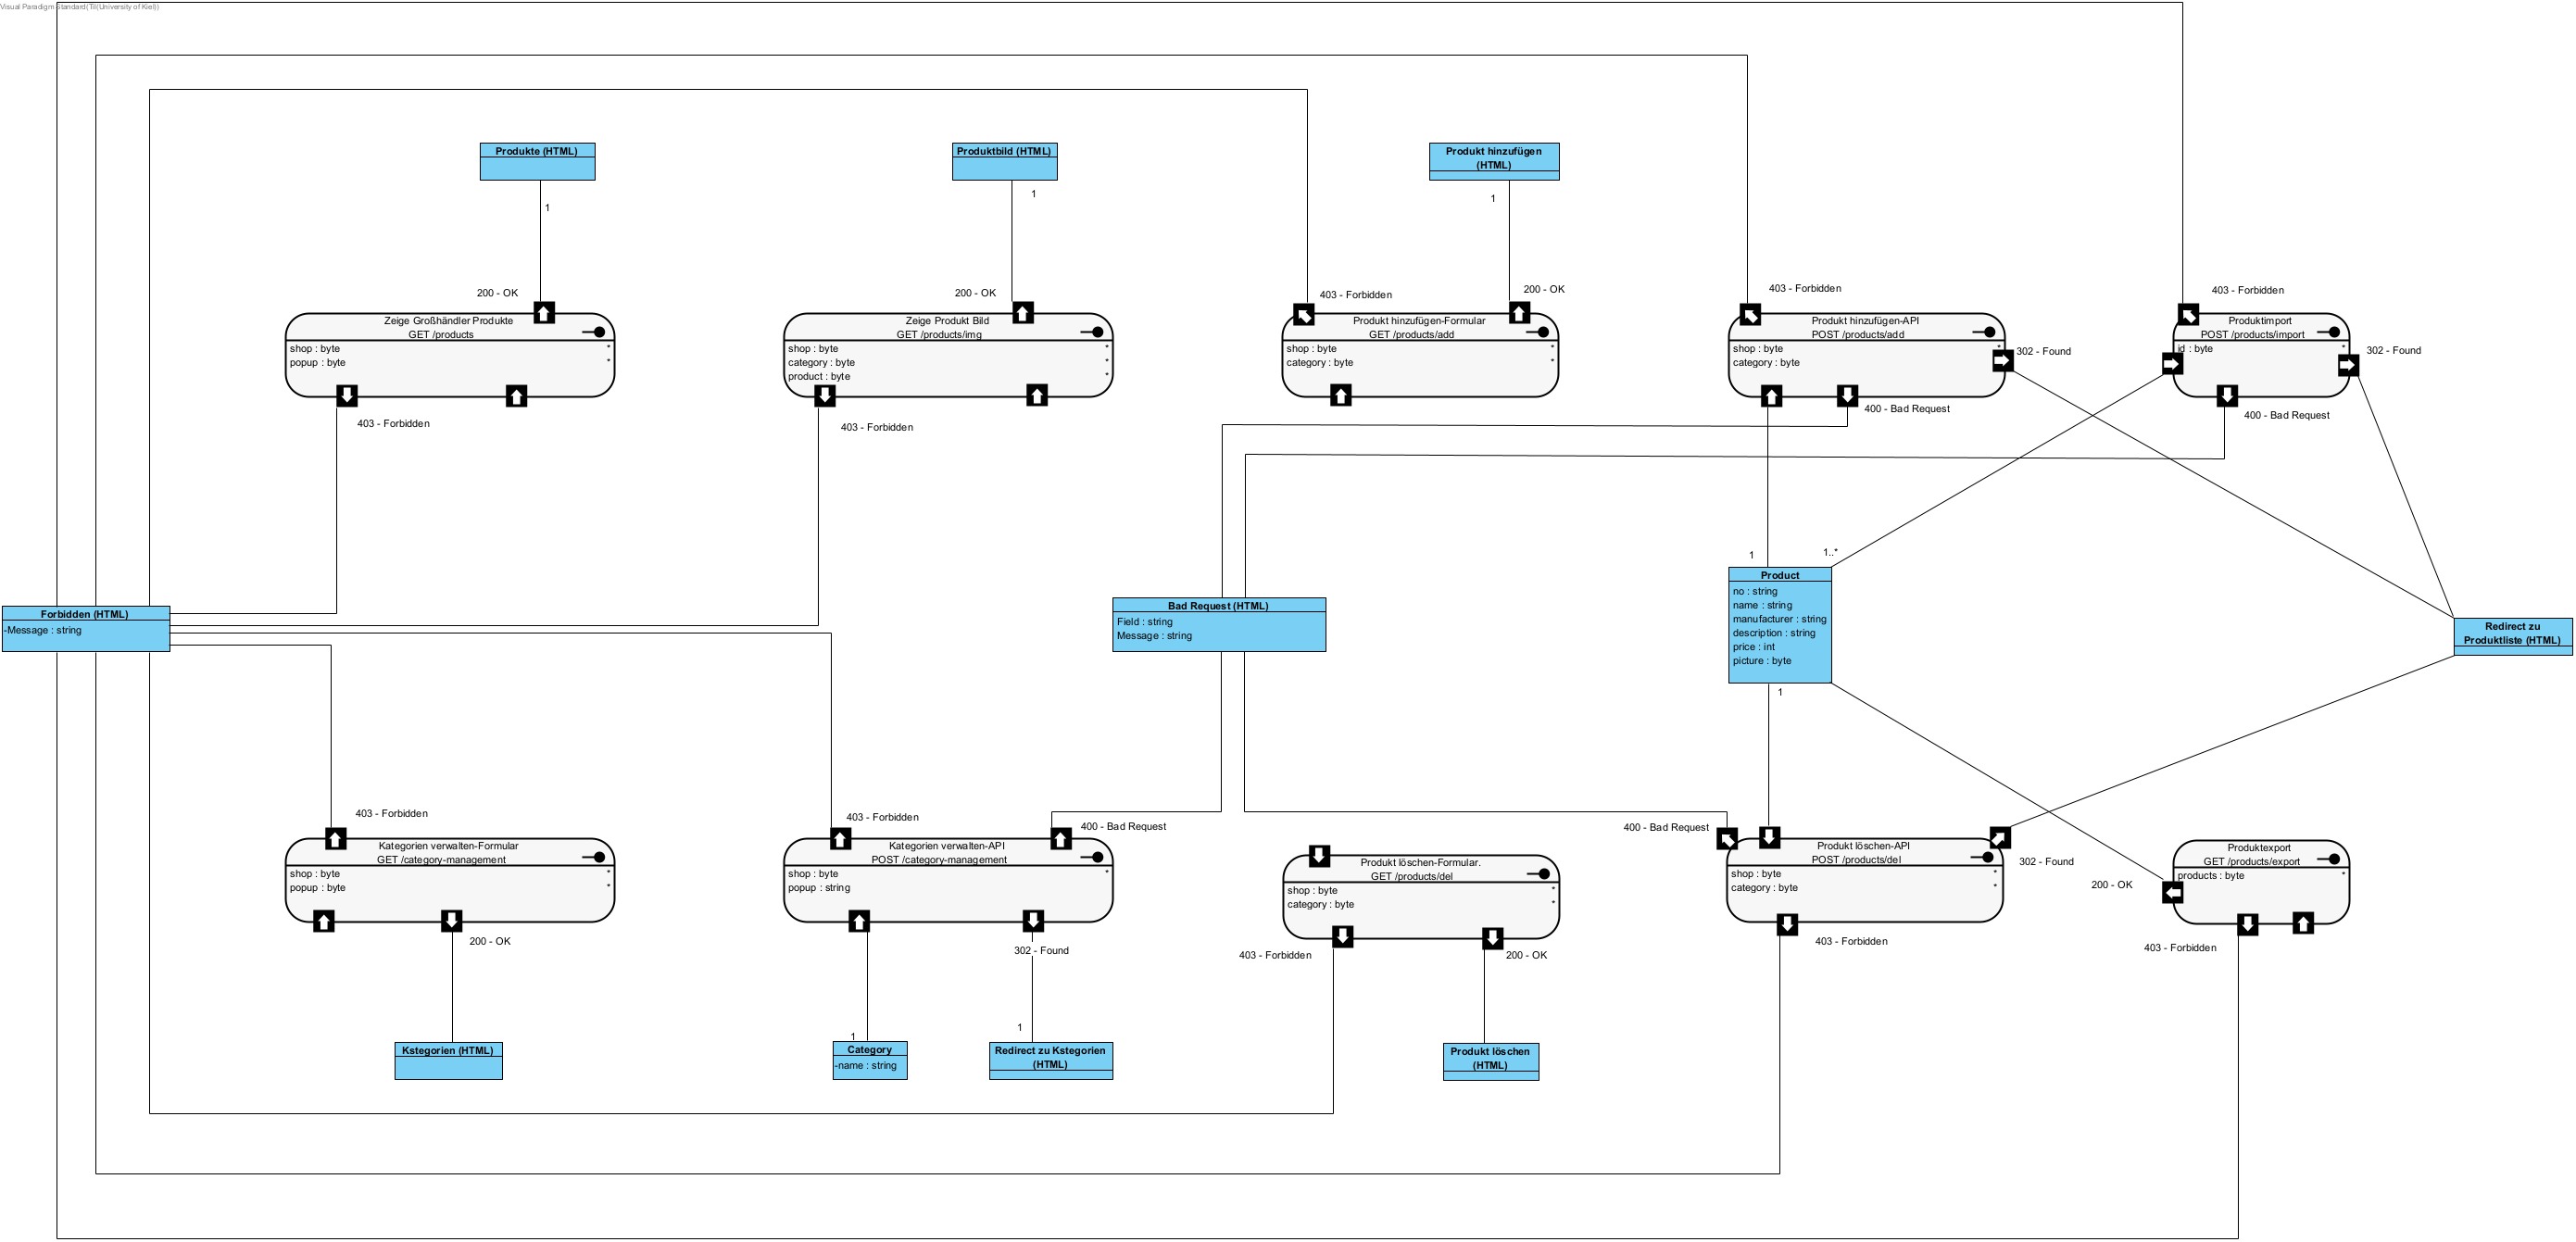
\includegraphics[width=\textwidth]{img/api-lehrkraft-produkt-kategorie}
Die folgenden Endpoints sind je nur mit einem Lehreraccount erreichbar, dessen Land zu evtl. angegebenen Großhändlern/Produkten passt.
\begin{itemize}
	\item \texttt{/products?shop=<ID>[\&category=<ID>\&popup=<ID>]}: Produktlisten aus Lehrkraft-Sicht.
		\begin{itemize}
			\item GET: Zeigt die Produktliste des angegeben Shops an. Je nach Parametern sind Produkte nach einer Kategorie gefiltert und/oder es wird ein Popup mit Text angezeigt.
		\end{itemize}
	\item \texttt{/products/img?product=<ID>}: Produktbilder.
		\begin{itemize}
			\item GET: Gibt als je natives Format das Bild des angegebenen Produktes zurück.
		\end{itemize}
	\item \texttt{/products/export?products=<ID>[,ID2[,ID3[...]]]}: Produktexport.
		\begin{itemize}
			\item GET: Gibt als JSON-Liste die angegebenen Produkte zurück.
		\end{itemize}
	\item \texttt{/products/import?shop=<ID>}: Produktimport.
		\begin{itemize}
			\item POST: Erwartet eine JSON-Liste an Produkten, die zu dem angegebenen Großhändler hinzugefügt werden.
		\end{itemize}
	\item \texttt{/products/add?shop=<ID>}: Produkt-Hinzufügungs-UI.
		\begin{itemize}
			\item GET: UI zum hinzufügen von einem Produkt.
			\item POST: Erwartet JSON mit Produktdaten \& Bild, und fügt es beim angegebenen shop in einer im JSON angegebenen Kategorie hinzu.
		\end{itemize}
	\item \texttt{/products/del?shop=<ID>}: Produktlöschungs-API.
		\begin{itemize}
			\item POST: Erwartet JSON mit Produkt-ID. Bei erfolg wird zu\\
				\texttt{/products?shop=ID\&popup=Erfolgreich+Gelöscht} weitergeleitet.
		\end{itemize}
	\item \texttt{/category-management?shop=<ID>[\&popup=<TEXT>]}: UI fürs hinzufügen/löschen von Kategorien.
		\begin{itemize}
			\item GET: UI zum Hinzufügen/Löschen von Kategorien, wobei man Änderungen erst speichern muss (was zu einem POST an dieselbe URL führt). Ein gegebenes Popup wird gezeigt.
			\item POST: Erwartet als JSON eine Liste an hinzugefügten \& gelöschten Kategorien. Bei Erfolg wird auf \texttt{/category-management?shop=ID\&popup=Erfolgreich+Geändert} weitergeleitet.
		\end{itemize}
\end{itemize}

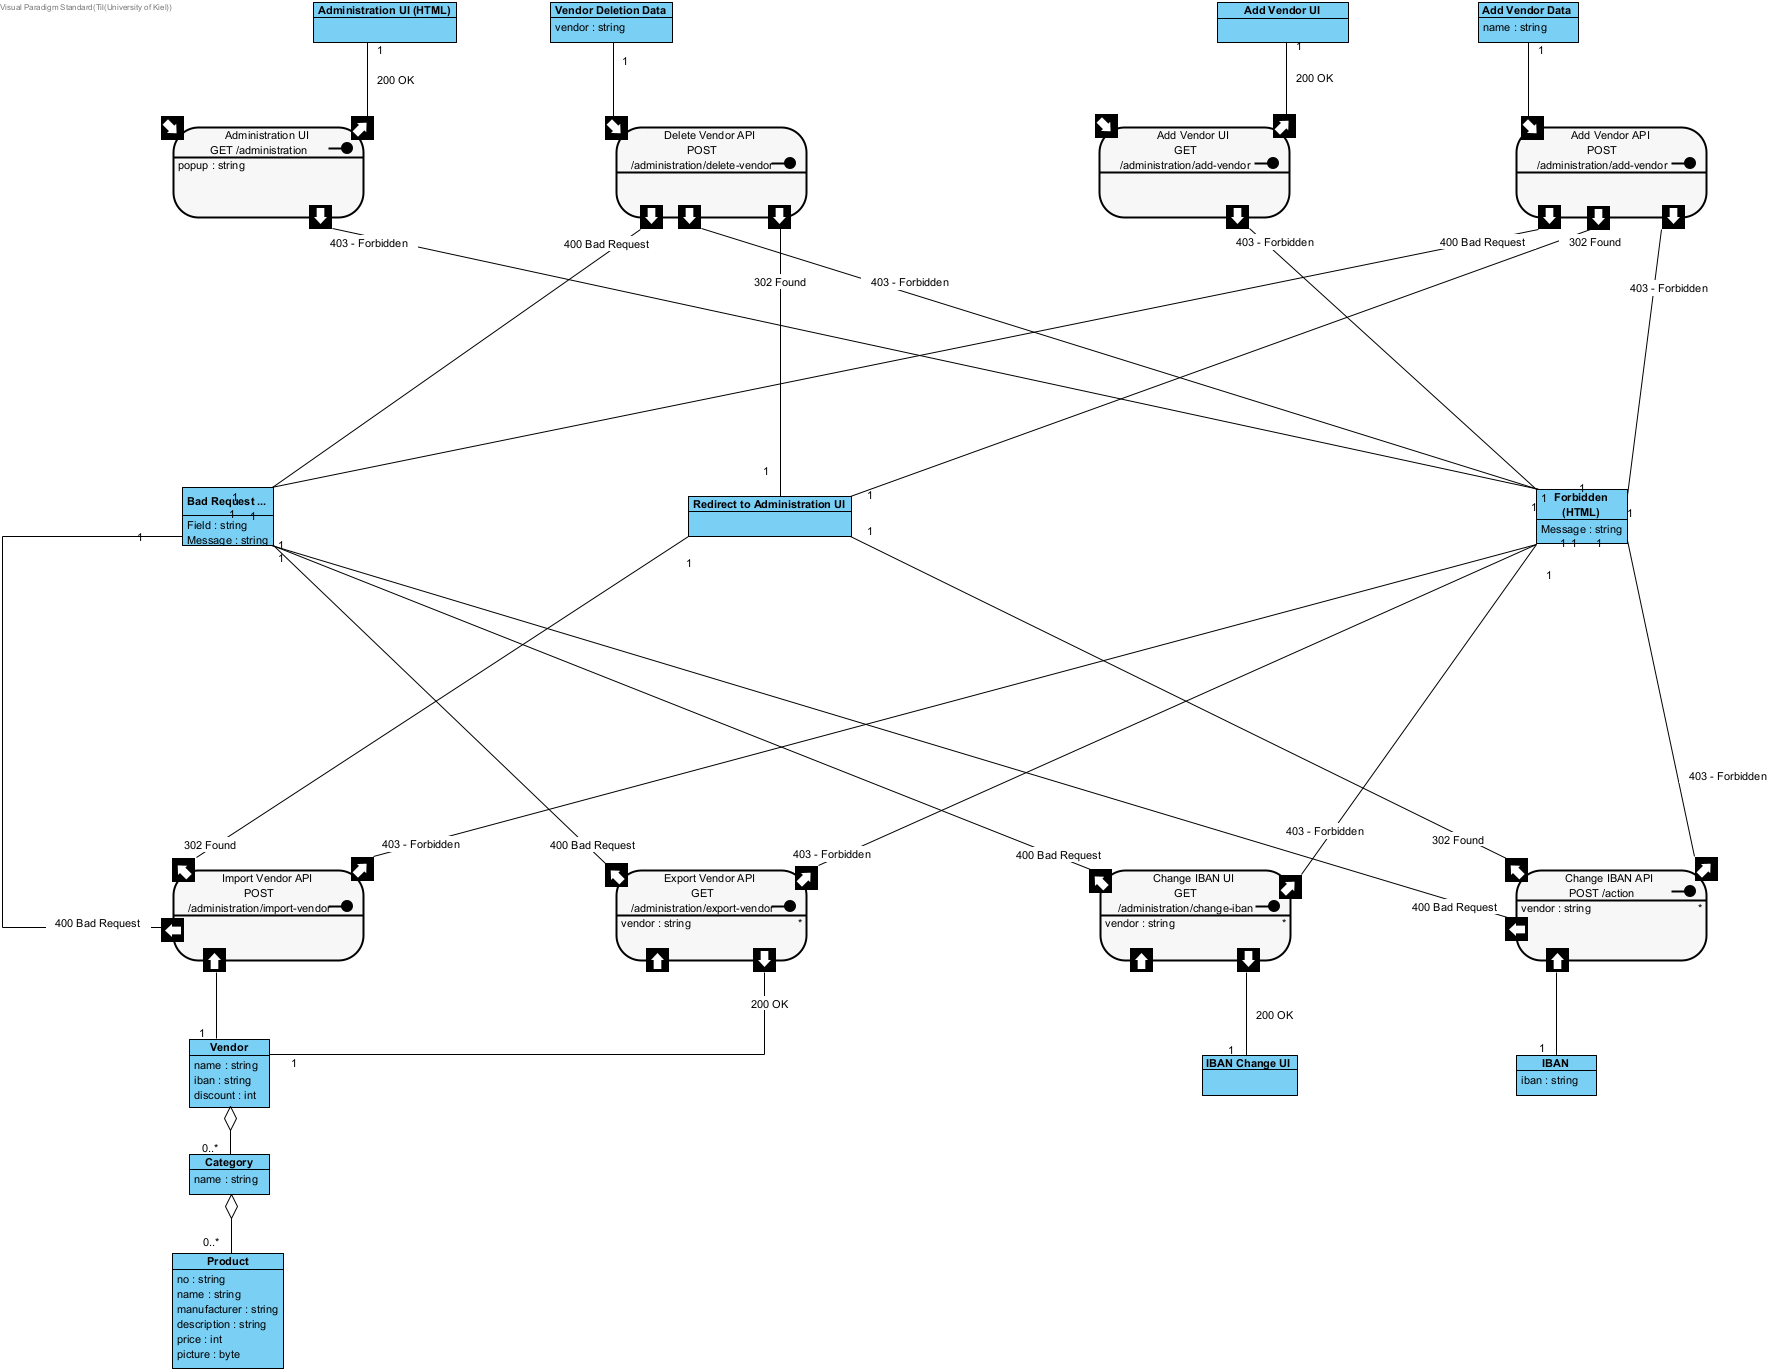
\includegraphics[width=\textwidth]{img/api-lehrkraft-administration}
\begin{itemize}
	\item \texttt{/administration?[popup=<TEXT>]}: UI zum verwalten von Großhändlern.
		\begin{itemize}
			\item GET: UI zum Hinzufügen/Löschen/Bearbeiten/Import/Export von Großhändlern. Ein gegebenes Popup wird gezeigt.
		\end{itemize}
	\item \texttt{/administration/add-vendor}: UI zum hinzufügen von vendors.
		\begin{itemize}
			\item GET: UI zum hinzufügen von Großhändlern.
			\item POST: Erwartet JSON mit Großhändler-Name, -Bild und -IBAN. Bei Erfolg wird auf \texttt{/administration?popup=Erfolgreich+Hinzugefügt} weitergeleitet.
		\end{itemize}
	\item \texttt{/administration/delete-vendor}: Großhändler-Löschungs-API.
		\begin{itemize}
			\item POST: Erwartet JSON mit Großhändler-ID, und löscht ihn \& zugehörige Produkte, Kategorien, Bestellungen \& Rechnungen. Bei Erfolg wird auf \texttt{/administration?popup=Erfolgreich+Gelöscht} weitergeleitet.
		\end{itemize}
	\item \texttt{/administration/export-vendor?shop=<ID>}: Großhändler-Export-API.
		\begin{itemize}
			\item GET: Gibt einen vendor mit allen Kategorien und Produkten, aber ohne zugehörigen Accounts und Bestellungen als JSON zurück.
		\end{itemize}
	\item \texttt{/administration/import-vendor}: Großhändler-Import-API.
		\begin{itemize}
			\item POST: Erwartet eine Datei, die durch einen Großhändler-Export erstellt wurde. Bei Erfolg wird auf \texttt{/administration?popup=Erfolgreich+Importiert} weitergeleitet.
		\end{itemize}
	\item \texttt{/administration/change-iban?shop=<ID>}: Großhändler-Bearbeitungs-UI.
		\begin{itemize}
			\item GET: Großhändler-Bearbeitungs-UI. Dabei sind auf jeden fall IBAN, später vielleicht auch das Logo einstellbar.
			\item POST: Erwartet JSON mit einer neuen IBAN und/oder einem neuen Logo. Bei Erfolg wird auf \texttt{/administration?popup=Erfolgreich+Geändert} weitergeleitet.
		\end{itemize}
\end{itemize}


\section{API-Diagramme für SuS}
Hier verzichten wir aufs Darstellen von Registrierung/Login, da es im wesentlichen gleich wie bei Lehrkräften aufgebaut ist, außer das alle pfade einen deeplink als Präfix haben.

\begin{itemize}
	\item \texttt{/<deeplink>}: Großhändlerübersicht-UI
		\begin{itemize}
			\item GET: UI, welche die Übersicht aller Großhändler des zugehörigen deeplinks anzeigt.
		\end{itemize}
	\item \texttt{/<deeplink>/invoice?id=<ID>}: Invoice-PDF
		\begin{itemize}
			\item GET: Zeigt Invoice als PDF an.
		\end{itemize}
	\item \texttt{/<deeplink>/catalog?[category=<ID>][\&popup=<TEXT>]}: Produktübersicht-UI
		\begin{itemize}
			\item GET: UI zur Übersicht der Produkte eines Großhändlers. Ein gegebenes Popup wird gezeigt.
		\end{itemize}
	\item \texttt{/<deeplink>/img?product=<ID>}: Produktbilder.
		\begin{itemize}
			\item GET: Gibt als je natives Format das Bild des angegebenen Produktes zurück.
		\end{itemize}
	\item \texttt{/<deeplink>/add-to-cart?[return-cat=<ID>]}: UI zum Hinzufügen von Produkten aus dem Warenkorb
		\begin{itemize}
			\item POST: Erwartet JSON mit Produkt-ID und Anzahl. Bei Erfolg wird auf \texttt{/<deeplink>/catalog?[category=<ID>]popup=Erfolgreich+Hinzugefügt} weitergeleitet.
		\end{itemize}
	\item \texttt{/<deeplink>/cat?[popup=<TEXT>]}: Warenkorb-UI
		\begin{itemize}
			\item GET: UI zur Ansicht des Warenkorbs. Ein gegebenes Popup wird gezeigt.
		\end{itemize}
	\item \texttt{/<deeplink>/del-from-cart}: UI zum Löschen von Produkten aus dem Warenkorb
		\begin{itemize}
			\item POST: Erwartet JSON mit Produkt-ID und löscht das Produkt. Bei Erfolg wird auf \texttt{/<deeplink>/car?popup=Erfolgreich+Gelöscht} weitergeleitet.
		\end{itemize}
	\item \texttt{/<deeplink>/checkout}: Bestellen-UI
		\begin{itemize}
			\item POST: Erwartet ein leeres JSON. Bei Erfolg wird auf die erstellte Invoice weitergeleitet.
		\end{itemize}
\end{itemize}

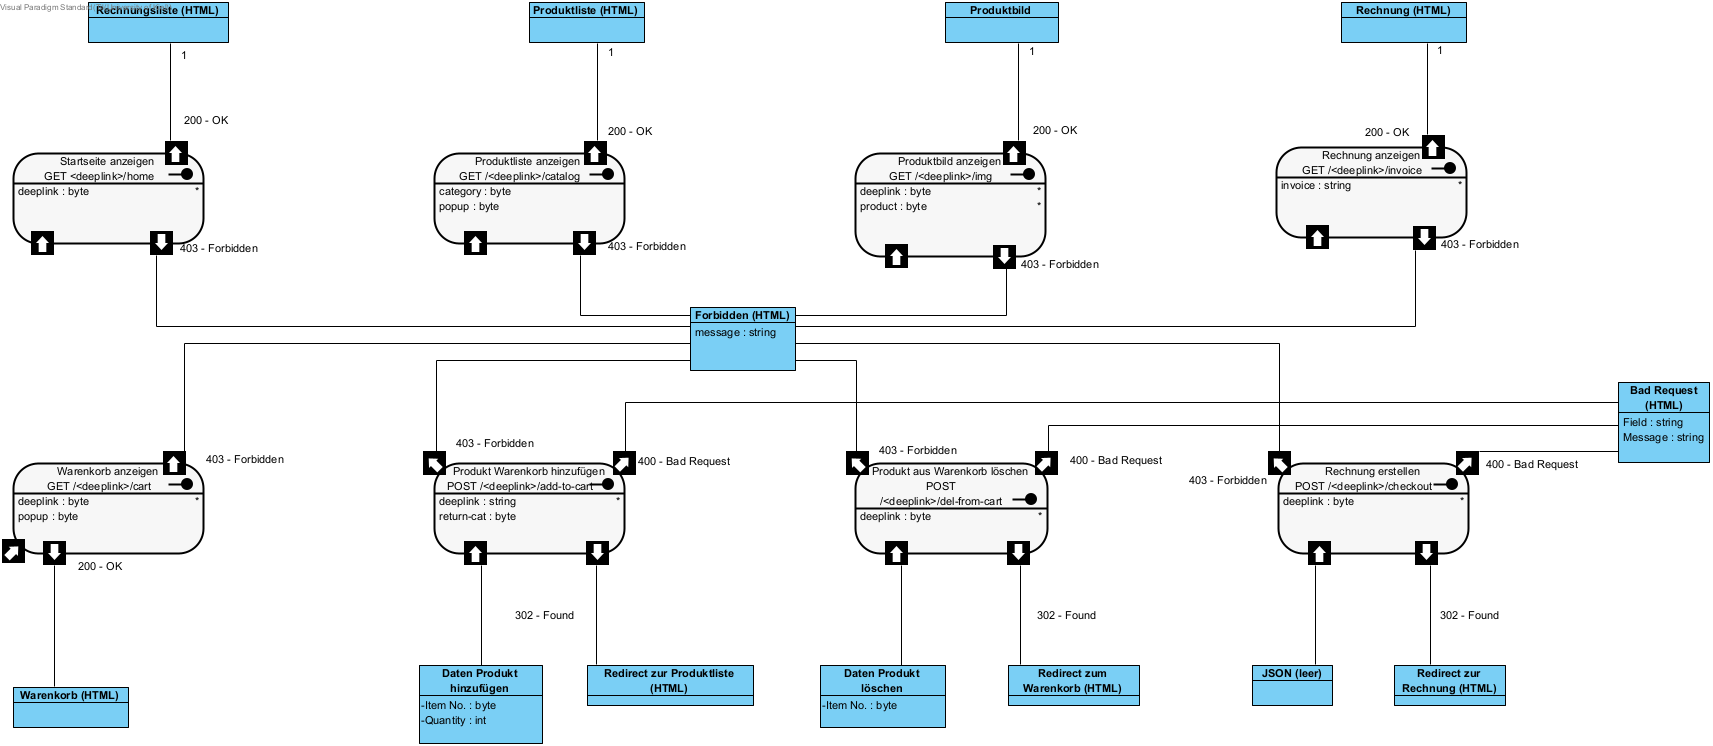
\includegraphics[width=\textwidth]{img/api-sus}
